
\documentclass[11pt,letterpaper]{article}

% Load some basic packages that are useful to have
% and that should be part of any LaTeX installation.
%
% be able to include figures
\usepackage{graphicx}
% get nice colors
\usepackage{xcolor}

% change default font to Palatino (looks nicer!)
\usepackage[latin1]{inputenc}
\usepackage{mathpazo}
\usepackage[T1]{fontenc}
% load some useful math symbols/fonts
\usepackage{latexsym,amsfonts,amsmath,amssymb}

% comfort package to easily set margins
\usepackage[top=1in, bottom=1in, left=1in, right=1in]{geometry}

% control some spacings
%
% spacing after a paragraph
\setlength{\parskip}{.15cm}
% indentation at the top of a new paragraph
\setlength{\parindent}{0.0cm}


\begin{document}

\begin{center}
\Large
Ay190 -- Worksheet 8\\
Anthony Alvarez\\
Date: February 6, 2014
\end{center}

\section{ODE Integration: Simplified Stellar Structure}

\subsection{Introduction}

We solve the system of two ODEs defined by hydrostatic equilibrium and mass
conservation. $$ \frac{dP}{dr} = - \frac{GM(r)}{r^2}\rho$$ and 
$$\frac{dM}{dr} = 4\pi\rho r^2$$. We define the polytropic equation of state
(EOS) to be $$P = K\rho^\Gamma$$ where $K$ is the polytropic constant 
and $\Gamma$
is the adiabatic index (the ratio of specific heats). In the following
computation we let these constants have values coresponding to a relativistically
degenerate white dwarf. $ K = 1.244 \times 10^{15} (0.5)^\Gamma dyne cm^{-2} (g
^{-1} cm^3)^\Gamma$ and $\Gamma = \frac43$

\subsection{Code Explanation}

The code found in ws8\_stellar\_structure.py is broken up into a few secions.
First we import relevant packages and then set up constants. Then we define 
helper functions that will simplify coding later. These include get\_rho
 which returns rho when given pressure, a stellar\_mass which 
returns the total mass of the star and self\_convergance which returns the order
of convergance for a given integrator.

The template also defined a few functions. The function tov\_RHS takes a radius,
pressure, density and mass and returns the list $[\frac{dP}{dr}, \frac{dM}{dr}, 
\rho]$ where $\rho$ is calculated by get\_rho. The integrators implement either
forward euler or RK integration of pressure and mass. 

The function stellar wraps some of the code in the template into a function. It
takes the number of grid points desired, the maximum radius desired and the 
integrator of choice and returns arrays of radius, pressure, density and mass
 enclosed as well as the index of the surface. It performs this by first 
setting up a grid and initializing arrays for pressure, rho and mass. Then it 
sets central values: rho is a constant $10^{10}$, pressure is determined from
the EOS and mass enclosed is initially 0. Then it sets up a termination
condiditon where the pressure falls below some critical value where the surface
of the star will be. Then It iterates forward with stepsize radmax/npoints and
integrates forward the pressure and mass and recaluclates rho based on those
values. If the pressure falls below the critical value then it sets the surface
index. 

\subsection{Testing the Code}

We filled in the sections in the code and when we ran it with a central density
$\rho_c = 10^{10} g cm^{-3}$, an outer radius of $2000 km$ and 500 grid points
we got the folloing values for each integration method. 

\begin{center}
\begin{tabular}{|c|c|c|}
\hline
\multicolumn{3}{|c|}{Mass and Radius Estimates}\\
\hline
Integration Method & $Mass_\odot$ & Radius \\
Forward Euler & 1.45069171385 & 1471.47147147\\
RK2 & 1.45748822161 & 1501.5015015 \\
RK3 & 1.4574213228 & 1501.5015015 \\
RK4 & 1.45742146222 & 1501.5015015 \\
\hline
\end{tabular}
\end{center}

\subsection{Convergance Factors}

By testing the code in low and high resolution, with (101, 201, 401) and (1001,
2001, 4001) points respectivly, we are able to get two different estimates for
 the conversion rate. The difference in low and high resolution is fairly low
except for the RK4. This difference is caused by the RK4 method hitting floating
point error at such high resolutions since it converges so quickly.

\begin{center}
\begin{tabular}{|c|c|c|}

\hline
\multicolumn{3}{|c|}{Conversion Factor}\\
\hline
Integration Method & Low Resolution & High Resolution \\
Forward Euler & 0.83 & 1.00 \\
RK2 & 2.11 & 2.01 \\
RK3 & 3.10 & 3.04 \\T

RK4 & 4.06 & 5.42 \\
\hline
\end{tabular}
\end{center}

\subsection{Plot of $\rho(r)$, $P(r)$, and$M(r)$}

We chose to plot a run using the RK3 inegrator at a resolution of 1000 points. 
In figure ~\ref{fig:pPM} we can see that pressure and density track each other 
reasonably well which makes sense given the EOS. It also appears the vast
majority of the mass of a star is contained in its inner $\frac13$ as the mass
attains almost its full value at around $500km$. 

\begin{figure}[bth]
\centering
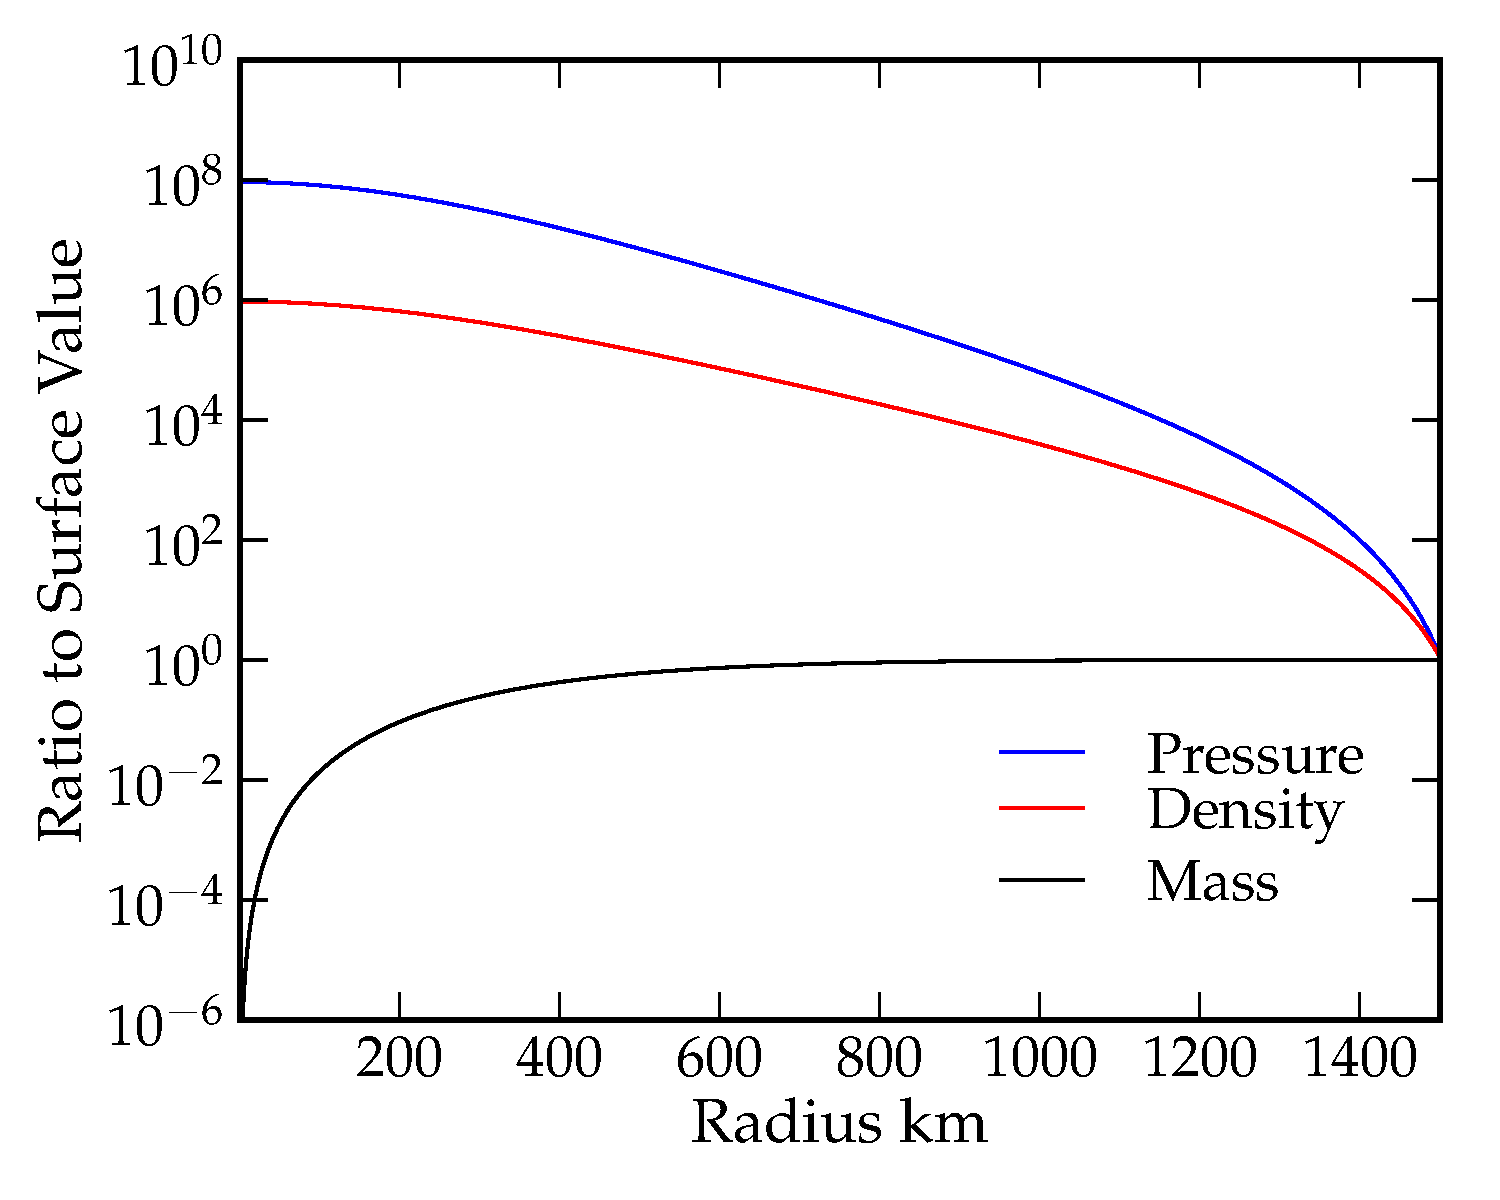
\includegraphics[width=0.5\textwidth]{4.pdf}
\caption{The average error from the true value for a given number of points.}
\label{fig:pPM}
\end{figure}


\end{document}




